\documentclass[8pt,mathserif,xcolor=dvipsnames]{beamer}
\usepackage{amsmath}
\usepackage{url}
\usepackage{enumerate}
\setbeamertemplate{navigation symbols}{}
\usepackage{helvet}
\usetheme{Warsaw} 
\usecolortheme[named=MidnightBlue]{structure}
\linespread{1.1}
\usepackage[T1]{fontenc}
\usepackage{listings}
\usepackage{color}
\usepackage{hyperref}
\definecolor{mybackground}{RGB}{250,250,250}
\definecolor{gray}{rgb}{0.5,0.5,0.5}
\definecolor{mauve}{rgb}{0.58,0,0.82}
\definecolor{dgreen}{rgb}{0,0.56,0}
\usepackage{listings}
\lstset{
language = python, % language
numbers = left, % where to put the line-numbers
numberstyle = \tiny, % the size of the fonts that are used for the line-numbers
stepnumber = 1, % the step between two line-numbers
numbersep = 6pt, % how far the line-numbers are from the code
backgroundcolor = \color{white},  % choose the background color, needs \usepackage{color}
showspaces = false, % show spaces adding particular underscores
showstringspaces = false, % underline spaces within strings
showtabs = false, % show tabs within strings adding particular underscores
frame = single, % adds a frame around the code
tabsize = 2,  % sets default tabsize to 2 spaces
captionpos = b, % sets the caption-position to bottom
breaklines = true, % sets automatic line breaking
breakatwhitespace = false, % sets if automatic breaks should only happen at whitespace
escapeinside = {\%*}{*)}, % if you want to add a comment within your code
basicstyle = {\footnotesize \ttfamily}, % define font size and style
showtabs = true,
showstringspaces = false,
keywordstyle = \color{magenta},
numberstyle = \tiny \color{dgreen},
commentstyle = \color{gray},
stringstyle = \color{mauve},
}
\setbeamertemplate{headline}
{
	\hbox
	{
	    \begin{beamercolorbox}[wd=.8\paperwidth,ht=.02cm,dp=1ex,left]{}
	    \end{beamercolorbox}
	}
}

% Adjust the itemize environment
\setbeamertemplate{itemize items}{$\bullet$}
\setbeamerfont{itemize/enumerate body}{size=\normalsize}
\setbeamerfont{itemize/enumerate subbody}{size=\normalsize}
\setbeamerfont{itemize/enumerate subsubbody}{size=\normalsize}

% Adjust the enumerate environment
\setbeamertemplate{enumerate items}{}

% Page number
\expandafter\def\expandafter\insertshorttitle\expandafter{%
  \insertshorttitle\hfill%
  \insertframenumber\,/\,\inserttotalframenumber}

\begin{document}

\setbeamercolor{background canvas}{bg=mybackground}

\title[Simbe]{Introducing Simbe for Technical Slides}
\subtitle{Simbe}
\author[JP Onnela]{JP Onnela}
\date[July 10, 2021]{July 10, 2021}
\institute[]{Department of Biostatistics \\ Harvard University}
\frame{\titlepage}

% ------------------------------------------------------------------------------------------------------------
\begin{frame}[fragile]
\frametitle{Introducing Simbe}
\begin{itemize}
	\item Simbe is an ultralight markup language for math / code heavy slides
	\item I wrote it in 2013 when I had to prepare 600+ slides for teaching a new course
	\item PowerPoint and Keynote were not feasible options for technical slides
	\item LaTeX Beamer has too much markup overhead for simple functionalities
	\item Simbe is a very simple LaTeX preprocessor written in Python 3
	\item It converts a Simbe file to a standard latex file which is compiled to PDF slides
	\item Simbe is short for Simple LaTeX Beamber
\end{itemize}

\end{frame}
% ------------------------------------------------------------------------------------------------------------
\begin{frame}[fragile]
\frametitle{Functionality of Simbe}
\begin{itemize}
	\item Simbe makes the following LaTeX / Beamer operations easy
	\begin{itemize}
	    \item Bullets
	    \item Equations
	    \item Figures
	    \item Code with syntax highlighting
	\end{itemize}
	\item These cover 99\% of my needs, but it's really just LaTeX, so you can do anything
	\item This is a famous equation:
\end{itemize}
\begin{equation}
E=mc^2
\end{equation}

\end{frame}
% ------------------------------------------------------------------------------------------------------------
\begin{frame}[fragile]
\frametitle{Figures}
\begin{itemize}
	\item Computers are now used everywhere in science
\end{itemize}
\begin{center}  \begin{figure}
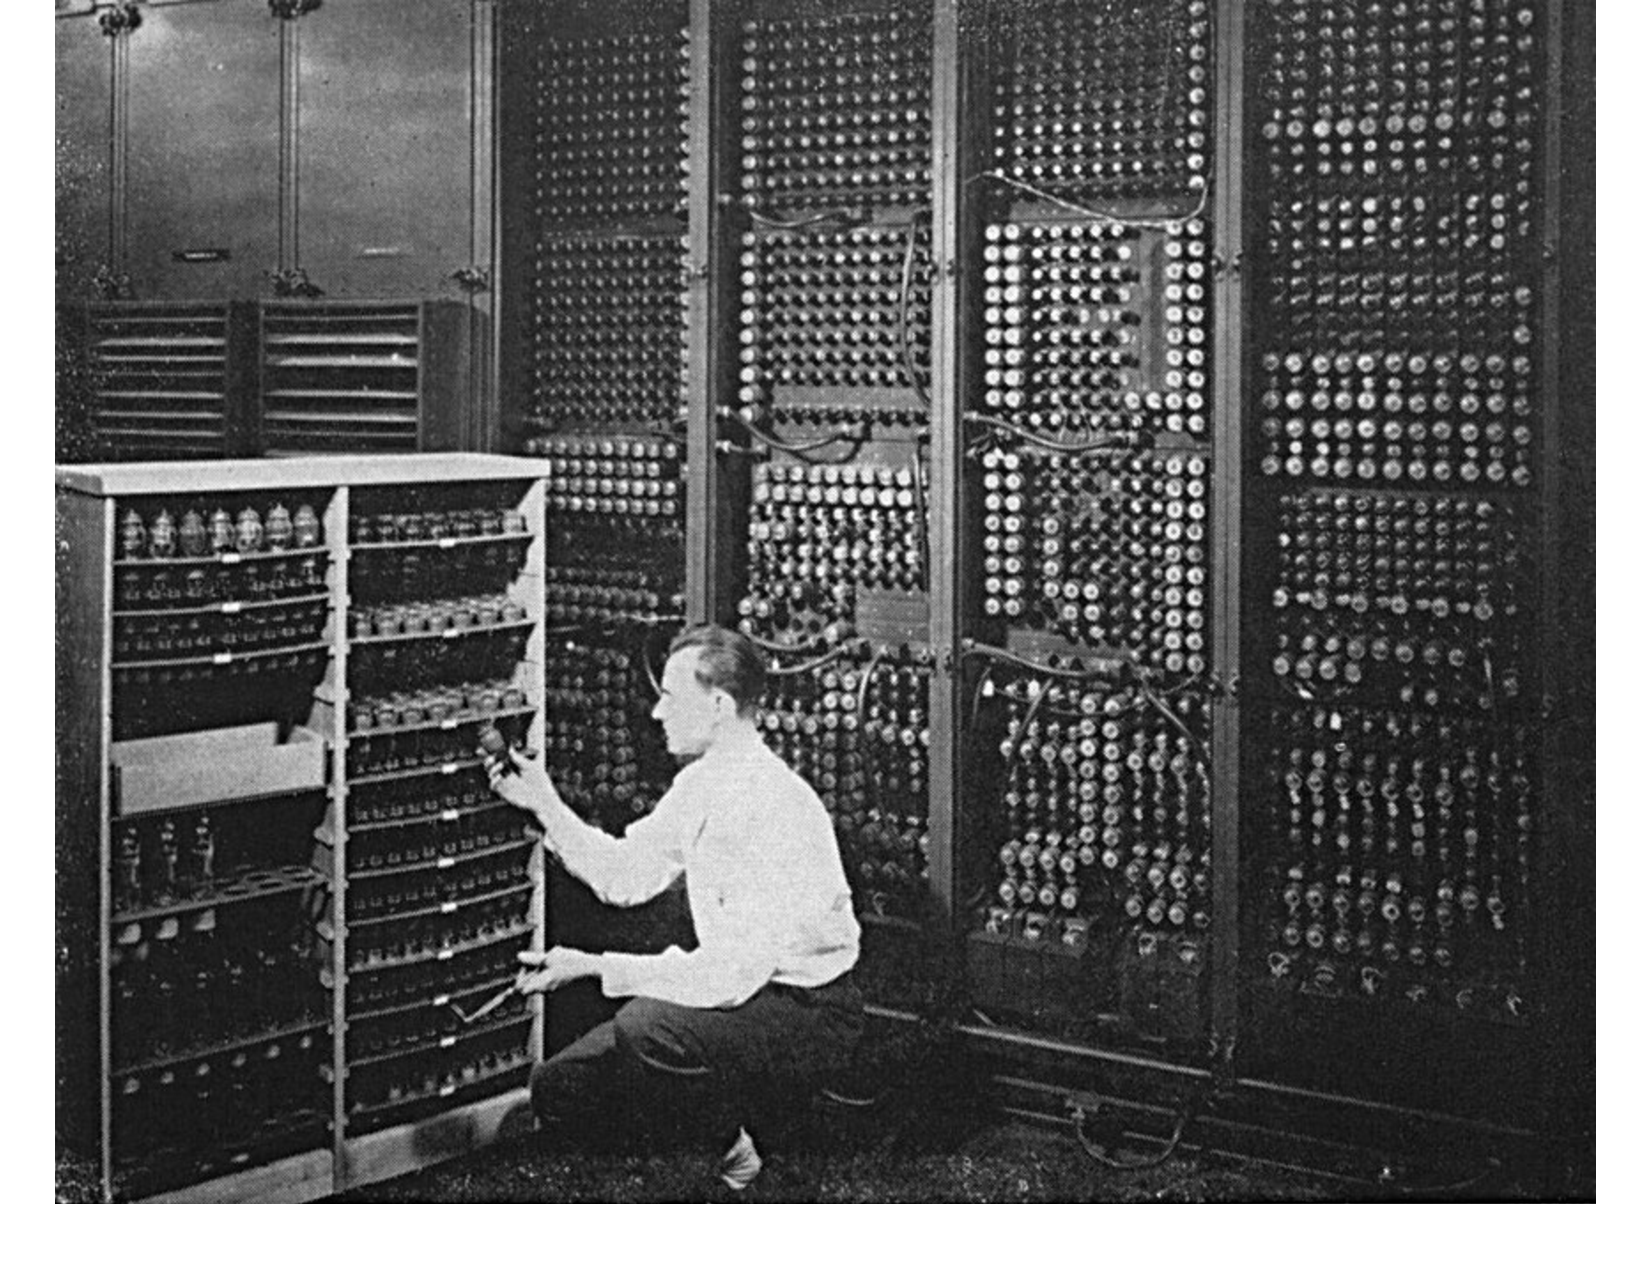
\includegraphics[width= 0.7\textwidth]{my-figure.pdf}
\caption{This is a serious computer.}
\end{figure}  \end{center}

\end{frame}
% ------------------------------------------------------------------------------------------------------------
\begin{frame}[fragile]
\frametitle{Code with Syntax Highlighting}
\begin{itemize}
	\item Python is increasingly used in research settings
	\item Check out my HarvardX course ``Using Python for Research''
	\item Here's a simple Python program with syntax highlighting:
\end{itemize}
\begin{lstlisting}
from math import pi
print(pi)
\end{lstlisting}

\end{frame}
% ------------------------------------------------------------------------------------------------------------
\begin{frame}[fragile]
\frametitle{Code with Syntax Highlighting}
\begin{itemize}
	\item Some programs are more complicated
	\item In some cases it's better to place a program in its own file
	\item It's especially heplful if you want to execute code on your slides
	\item Here's Python code for generating the Fibonacci sequence
\end{itemize}
\lstinputlisting{my_code.py}

\end{frame}
% ------------------------------------------------------------------------------------------------------------
\end{document}
